\section{Zusammenfassung und Diskussion}

Werden die elementaren elektronischen Bauteile Widerstand, Kondensator und Spule gemeinsam in einem Schaltkreis verbunden, weisen diese für unterschiedliche Konfigurationen besondere Verhaltensweisen im Zusammenhang mit Wechselspannung auf. RC-Glieder, also Schaltungen aus einem Widerstand und einer Spule können beispielsweise als Hoch- oder Tiefpassfilter verwendet werden, während das Hinzuschalten einer Spule einen Schwingkreis erzeugt. Derartige Schaltungen waren das Zentralversuchsobjekt in Versuch 241.

Im ersten Versuchsteil haben wir ein RC-Glied betrachtet. Hierzu haben wir für verschiedene Werte von Kapazität und Widerstand haben wir die Zeitkonstante $\tau$ zunächst aus unseren Beobachtungen am Oszilloskop bestimmt und zum Vergleich den zugehörigen theoretisch vorausgesagten Wert berechnet. Die Werte sind in der untenstehenden \tabref{tab:zsmf_a1_zeitkonst} noch einmal zusammengefasst.


\renewcommand{\arraystretch}{1.5}
\begin{table}[H]
  \centering
  \caption{Messwerte und berechnete Größen der Zeitkonstante $\tau$.}
  \vspace*{1em}
  \begin{tabular}{| c | c | c | c | c |}
      \hline
      $C\ [\si{\nano\farad}]$ & $R\ [\si{\kilo\ohm}]$ & $\tau_{\text{theo}}\  [\si{\second}]$ & $\tau_{\text{exp}}\ [\si{\second}]$ & Abw. \\
      \hline
      $470$ & $1.00$ & $(47 \pm 6) \times 10^{-5}$ & $(43 \pm 15) \times 10^{-5}$ & $0.25\sigma$ \\
      \hline
      $4.70$ & $10.00$ & $(4.7 \pm 0.6) \times 10^{-5}$ & $(6.49 \pm 0.15) \times 10^{-5}$ & $3.29\sigma$ \\
      \hline
      $47.00$ & $1.00$ & $(4.7 \pm 0.6) \times 10^{-5}$ & $(4.91 \pm 0.15) \times 10^{-5}$ & $0.38\sigma$ \\
      \hline
  \end{tabular}
  \label{tab:zsmf_a1_zeitkonst}
\end{table}
\renewcommand{\arraystretch}{1}

Es ist zu sehen, dass in zwei von drei Fällen der gemessene Wert sehr gut mit dem theoretisch vorhergesagten Wert übereinstimmt. Die sehr starke Abweichung bei der Konfiguration mit $C = 4.7\si{\nano\farad}, R = 10\si{\kilo\ohm}$ fällt deutlich heraus und ist vermutlich auf einen groben Messfehler oder einen Fehler in den verwendeten Bauteilen zurückzuführen.

Im zweiten Versuchsteil haben wir qualitativ die Wirkung eines RC-Gliedes als Differentiator und Integrator untersucht. Je nachdem, ob wir die Ausgangsspannung am Kondensator oder am Widerstand abgenommen haben, hat diese in etwa die Form des differenzierten bzw. integrierten Eingangssignals dargestellt. Durch Manipulation des Widerstandes mithilfe eines Potentiometers konnten wir bestätigen, dass dieser Wert eine maßgebliche Auswirkung auf die Annäherung des Ausgangssignals an die entsprechende Form hat.

RC-Schaltungen wirken für eingehende Signale wie ein Hoch- oder Tiefpassfilter, je nachdem ob die Ausgangsspannung über den Kondensator oder die Spule abgegriffen wird. Den Frequenz- und Phasengang dieser Filterschaltungen haben wir im dritten Versuchsteil untersucht. Mithilfe der Oszilloskopsoftware haben wir die Frequenzgänge je für eine Tiefpass- und eine Hochpassfilterschaltung aufgezeichnet. Aus den Frequenzgängen haben wir die Grenzfrequenz, also die Frequenz ab welcher die Wirkung des Filters greift bestimmt. Hierbei haben wir einen Wert von 
\begin{gather*}
  f_{G,TP} = (9.46 \pm 0.02)\si{\kilo\hertz}
  \intertext{für den Tiefpassfilter und}
  f_{G,HP} = (3.31 \pm 0.02)\si{\kilo\hertz} 
\end{gather*}
für den Hochpassfilter gemessen. Für den Hochpassfilter haben wir uns zusätzlich dazu noch den Phasengang angeschaut. Da dieser nicht automatisch von der Oszilloskopsoftware aufgezeichnet werden konnte, haben wir diesen manuell aus der zeitlichen Verschiebung von Ein- und Ausgangssignal gemessen. Die Messung haben wir für verschiedene Frequenzen durchgeführt und die resultierenden Phasen darüber in ein Diagramm aufgetragen. Durch eine Interpolation der gemessenen Werte haben wir dann die Frequenz bei einer Phase von $45\si{\degree}$ und damit einen zweiten Wert für die Grenzfrequenz bestimmt. Dieser beläuft sich auf
\begin{align*}
  f_{G,HP,\varphi} &= (3.65 \pm 1.48)\si{\hertz} 
\end{align*}
und weicht damit um etwa $2.47\sigma$ vom zuvor bestimmten Wert ab. Aus der Vorhersage der Theorie haben wir für die Grenzfrequenz einen Wert von
\begin{align*}
  f_{G,theo} &= (3.4 \pm 0.4)\si{\kilo\hertz}
\end{align*}
berechnet. Mit einer Abweichung von nur etwa $0.21\sigma$ liegt dieser Wert sehr nah an dem Wert, welchen wir aus dem Frequenzgang bestimmt haben. Die Abweichung zum aus dem Phasengang interpolierten Wert ist mit etwa $2.47\sigma$ wieder sehr hoch. Die starke Abweichung des interpolierten Wertes von den zwei anderen lässt sich vermutlich einerseits auf Messungenauigkeiten bei der Vermessung der Phasenverschiebung, sowie den Fehler aus der Interpolation zurückführen.

Aufgrund des in der Auswertung genannten Fehlers bei der Aufzeichnung der Frequenzgänge lohnt sich ein Vergleich mit der Grenzfrequenz des Tiefpassfilters nicht.

Im vierten Aufgabenteil haben wir durch Hinzuschalten einer Spule erstmals ein RLC-Glied betrachtet. Für eine eingehende Wechselspannung wirkt ein RLC-Glied wie ein Bandpassfilter, also eine Kombination aus einem Hoch- und einem Tiefpassfilter. Für drei unterschiedliche Werte des Widerstandes haben wir Ein- und Ausgangsamplitude, sowie die Resonanzfrequenz und die Bandbreite der Filterschaltung gemessen. Aus Resonanzfrequenz haben wir dann zusammen mit der Kapazität des verbauten Kondensators die Induktivität der Spule zu
\begin{align*}
  L = (3.63 \pm 0.22) \cdot 10^{-2}\si{\henry}
\end{align*}
bestimmt. Daraufhin haben wir die durch die Spule verursachten Verluste in der RLC-Schaltung untersucht. Um diese zu quantifizieren haben wir die Existenz eines zusätzlichen Verlustwiderstandes $R_V$ angenommen, mit welchem sich der Gesamtwiderstand der Schaltung auf $R + R_V$ beläuft. Den Gesamtwiderstand haben wir dann auf zwei verschiedenen Wegen, über die Bandbreite und die Induktivität, sowie über das Verhältnis der von Ein- und Ausgangsspannung bestimmt. In \tabref{tab:zsmf_verlustwiderstand} sind die Resultate der beiden Rechenwege noch einmal zusammengefasst dargestellt.

\renewcommand{\arraystretch}{1.5}
\begin{table}[H]
  \centering
  \caption{Resultate und Abweichungen für die Berechnung des Verlustwiderstandes.}
  \vspace*{1em}
  \begin{tabular}{|c|c|c|c|c|}
    \hline
    \multicolumn{2}{|c|}{$R\,[\si{\ohm}]$} & $1000 \pm 50$ & $220 \pm 11$ & $47.0 \pm 2.4$ \\
    \hline
    \hline
    \multirow{2}{*}{Aus Bandbreite} & $R + R_V\,[\si{\ohm}]$ & $1123 \pm 650$ & $294 \pm 171$ & $128 \pm 75$ \\
    \cline{2-5}
    & $R_V\,[\si{\ohm}]$ & $123 \pm 652$ & $74 \pm 171$ & $80 \pm 75$ \\
    \hline
    \hline
    \multirow{2}{*}{Aus Amplituden} & $R + R_V\,[\si{\ohm}]$  & $1033 \pm 61$ & $270 \pm 17$ & $109 \pm 10$ \\
    \cline{2-5}
    & $R_V\,[\si{\ohm}]$ & $33 \pm 79$ & $49.811 \pm 21$ & $62.144 \pm 11$ \\
    \hline\hline
    \multicolumn{2}{|c|}{Abweichung} & $0.792\sigma$ & $0.838\sigma$ & $1.296\sigma$ \\\hline
  \end{tabular}
  \label{tab:zsmf_verlustwiderstand}
\end{table}
\renewcommand{\arraystretch}{1}

Die Abweichungen zwischen den Resultaten der beiden Rechenwege sind mit Größen um $1\sigma$ relativ gering und vermutlich hauptsächlich auf Messungenauigkeiten zurückzuführen. Dass der Verlustwiderstand der Spule über die verschiedenen Widerstandswerte nicht konstant ist, hängt damit zusammen, dass dieser frequenzabhängig ist. Wie auch in der Auswertung dieser Aufgabe zu sehen, ergeben sich für die verschiedenen Widerstände ganz verschiedene Frequenzgänge der Schaltung.

Weiter mit dem Serienschwingkreis haben wir im nächsten Schritt die Frequenzgänge aller drei Bauteile untersucht. Eine Besonderheit bei Betrachtung der Frequenzgänge von Kondensator und Spule ist, dass es bei diesen zu einer sogenannten Resonanzüberhöhung kommt. Dabei steigt bei der jeweiligen Resonanzüberhöhung der Bauteile der Wert der Ausgangsamplitude über den Wert der Eingangamplitude an. Dies konnten wir sehr gut an den aufgezeichneten Frequenzgängen beobachten. Aus diesen haben wir dann für alle drei Bauteile die jeweilige Resonanzfrequenz abgelesen. Um diese mit der theoretischen Voraussage zu vergleichen haben wir zunächst die Dämpfungskonstante des Schwingkreises auf
\begin{align*}
  \delta = (3028 \pm 1758)\si{\per\second}
\end{align*}
bestimmt. Damit konnten wir die Resonanzfrequenz des Widerstandes, und mithilfe dieser wiederum die Resonanzfrequenzen von Kondensator und Spule berechnen. Die Werte sind zum Vergleich in \tabref{tab:zmf_omega_vergleich} zusammengefasst.


\renewcommand{\arraystretch}{1.5}
\begin{table}[H]
  \centering
  \caption{Vergleich der gemessenen und theoretisch vorhergesagten Werte der Resonanzfrequenzen der Bauteile im RLC-Serienschwingkreis.}\vspace*{0.5em}
  \label{tab:zmf_omega_vergleich}
  \begin{tabular}{|l|c|c|c|}
    \hline
    & $\omega_R\,[\si{\per\second}]$ & $\omega_C\,[\si{\per\second}]$ & $\omega_L\,[\si{\per\second}]$\\\hline
    Gemessener Wert & $3910 \pm 20$ & $3800 \pm 20$ & $4040 \pm 20$ \\\hline
    Theoretischer Wert & $3851 \pm 1131$ & $3791 \pm 1149$ & $3911 \pm 1114$\\\hline\hline
    Abweichung & $0.06\sigma$ & $0.009\sigma$ & $0.12\sigma$\\
    \hline
  \end{tabular}
\end{table}
\renewcommand{\arraystretch}{1}

Die Fehler der theoretisch Werte sind sehr groß, was ein Grund für die sehr geringe $\sigma$-Abweichung zwischen diesen und den gemessenen Werten ist. Andererseits fällt auch bei Betrachtung der absoluten Unterschiede auf, dass die Theorie sehr nahe an der Praxis ist.

Bevor wir zum mehr praxisorientierten Teil fortgefahren sind, haben wir noch einmal kurz einen Parallelschwingkreis betrachtet. Auch für diesen haben wir einen Frequenzgang aufgezeichnet, in welchem sich sehr gut das Einsetzen der Bandsperre bei der Resonanzfrequenz beobachten ließ. Aus dem Grafen haben wir eine Resonanzfrequenz von 
\begin{align*}
  f_{0,exp} = (3.94 \pm 0.02)\si{\kilo\hertz}
\end{align*}
abgelesen. Die Theorie sagt für die verwendete Konfiguration eine Resonanzfrequenz von 
\begin{align*}
  f_{0,theo} = (3.85 \pm 1.14)\si{\kilo\hertz}
\end{align*}
voraus. Diese weicht um gerade mal $0.078\sigma$ vom gemessenen Wert ab. Auch hier ist wieder ein großer Fehler im theoretischen Wert für die außergewöhnlich geringe $\sigma$-Abweichung verantwortlich. Allerdings zeigt ein direkter Vergleich der Werte ebenso eine sehr gute Annäherung.

In Aufgabe 8 haben wir uns dann erstmalig mit einer tatsächlichen praktischen Anwendung der RC- und RLC-Glieder auseinandergesetzt. Mit dem Funktionsgenerator haben wir ein Sinussignal aus mehreren überlagerten verschiedenen Frequenzen generiert. Dessen Spektrum sah zunächst wie in \abbref{fig:zmfs_aufgabe8_teil1_osz} zu sehen aus. Die primären Anteile waren ein $100\si{\hertz}$-, ein $4\si{\kilo\hertz}$- und ein $8\si{\kilo\hertz}$-Signal, welche auch leicht im ungefilterten Spektrum zu sehen sind.

\begin{figure}[H]
  \centering
  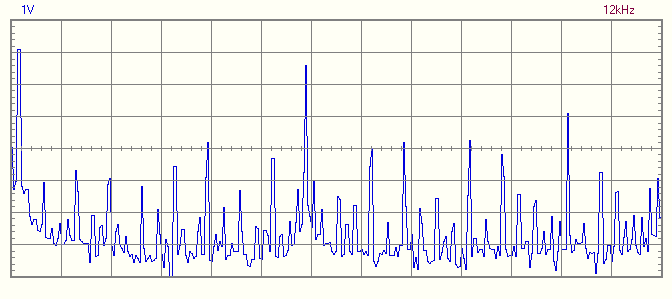
\includegraphics[width=.8\textwidth]{files/aufgabe8_teil1_spectrum.png}
  \caption{Frequenzspektrum des überlagerten Signals ohne Filter.}
  \label{fig:zmfs_aufgabe8_teil1_osz}
\end{figure}

Mit dem Ziel, den mittig zu sehenden Anteil bei in etwa $4\si{\kilo\hertz}$ zu isolieren und alle umliegenden Frequenzen weitestgehend zu dämpfen haben wir das Signal durch verschiedene Schaltungen gefiltert. Dazu gehörten RC-Hoch- und Tiefpassfilter, ein LC-Tiefpassfilter, sowie verschiedene Konfigurationen des RLC-Bandpassfilters. Die beste Herausstellung des $4\si{\kilo\hertz}$-Anteils, zu sehen in \abbref{fig:zsmf_aufgabe8_teil3_clR_47ohm_bandpass}, konnten wir mit einem RLC-Bandpassfilter mit einem $47\si{\kilo\ohm}$ Widerstand erzielen. Die Ausgangsspannung haben wir hier am Widerstand abgenommen.

\begin{figure}[H]
  \centering
  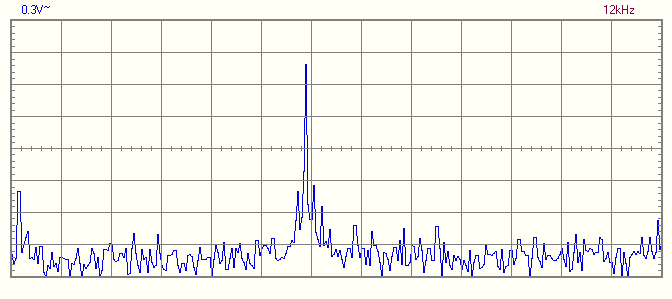
\includegraphics[width=.8\textwidth]{files/aufgabe8_teil3_clR_47ohm_bandpass_spectrum.png}
  \caption{Frequenzspektrum des überlagerten Signals mit $RLC$-Bandpassfilter mit $47\si{\kilo\ohm}$ Widerstand, bei Spannungsabnahme über den Widerstand.}
  \label{fig:zsmf_aufgabe8_teil3_clR_47ohm_bandpass}
\end{figure}

Wie im Spektrum zu sehen, haben wir in diese Konfiguration den $8\si{\kilo\hertz}$-Anteil so weit herausgefiltert, dass dieser komplett im Untergrund verschwindet. Der $4\si{\kilo\hertz}$ wurde ebenfalls sehr stark gedämpft. Bei einem Vergleich der gefilterten und ungefilterten Amplitude haben wir für diesen eine Dämpfung von
\begin{align*}
  \delta_{100\si{\hertz}} = 0.0532 \pm 0.0004
\end{align*}
berechnet. Besonders gut zu sehen ist in diesem Spektrum nun der $4\si{\kilo\hertz}$-Anteil. Diese erfuhr durch die Filterschaltung eine Dämpfung von
\begin{align*}
  \delta_{4\si{\kilo\hertz}} = 0.4357 \pm 0.0012.
\end{align*}

Als zweites Anwendungsgebiet haben wir mit einer RLC-Schaltung einen AM-Empfänger simuliert. Über eine Sendeantenne im Versuchsraum wurde ein kontinuierliches Sinussignal ausgesendet. Dieses haben wir über eine Antenne empfangen und versucht, es durch die Filterschaltung möglichst störungsfrei am Oszilloskop anzuzeigen. Dabei haben wir außerdem die Auswirkungen der Variation der Kapazität im Schwingkreis, sowie eines Eisenkerns  in der Spule qualitativ beobachtet.

Wir konnten beobachten, dass die Amplitude des empfangenen Signals bis zu einem Maximum mit Erhöhung der Kapazitäten zu- und dann wieder abnahm. Beim Entfernen des Eisenkerns aus der Spule konnten wir eine Abnahme der Amplitude beobachten. Tatsächlich schafften wir es, durch etwas fine-tuning an der Filterschaltung ein nur noch leicht verzerrtes Sinussignal am Oszilloskop anzuzeigen.

Weiter versuchten wir ein tatsächliches Audiosignal, welches im Raum durch einen Spulenaufbau ausgesendet wurde, zu empfangen und mit der Filterschaltung aufzulösen. Leider schlugen hierbei all unsere Versuche fehl und wir haben es nicht geschafft, ein über Kopfhörer hörbares Signal zu bekommen.